
\section*{First Design}
The first design considered is a basic IIR filter with a critical delay path of one multipler and one adder. This design includes a simple data truncation at the output Y[N] such that the lower order bits are discarded completely. Refer to Figure \ref{subfig:block1-a} for the general block diagram. operands are eight bits, outputs of the multipliers are sixteen bits, and all adders are sixteen bit. The input and output waveforms, see Figure \ref{subfig:output1-b}, indicate that this design is not optimal, however, we will see that further optimization also had little impact on this initial result.

\subsection*{First Verilog Code Iteration}
Take note that no reset signal is needed. This reseting is handled by modeling a weak pull-down in the registers. In the event that the input value is unknown or high impedence, the output value defaults to zero. This helps to reduce the port list and also internal routing required for this control signal. 
\\*
\lstset{language=verilog}
\lstinputlisting[caption=First Iteration, label=lst:first_code]{projfilt.v}
\subsection*{Truncation Code}
The code used in the first design to truncate the lower order bits simply only sends the higher order eight bits to the output.\\*
\\*
always @ (posedge clk)\\*
begin	\\*
y = d3[15:8];\\*
end\\*

\subsection*{First Design Timing Analysis}

% Table generated by Excel2LaTeX from sheet 'Sheet1'
\begin{table}[bh]
\caption{Xilinx Timing Report}
\begin{tabular}{c|c}
\centering
           & Timing in (ns) \\
\hline
     Delay &     18.684 \\

Requrement &        100.000 \\

Data Path Delay &     18.538 \\
\end{tabular}  
\label{tab:timing1}
\end{table}

According to Table \ref{tab:timing1}, the maximum clock frequency for this design has been calculated to be approximately: 53.5 MHz.

\begin{figure}[htp]
  \begin{center}
    \subfigure[Functional block diagram]{\label{subfig:block1-a}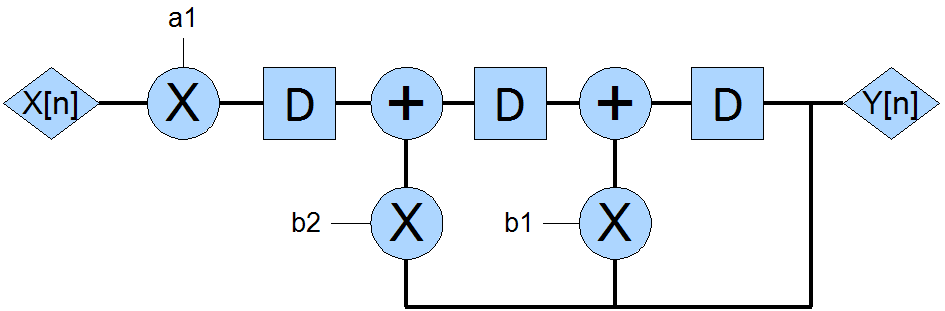
\includegraphics[scale=0.30]{block_one.png}}
    \subfigure[Input/Output comparison]{\label{subfig:output1-b}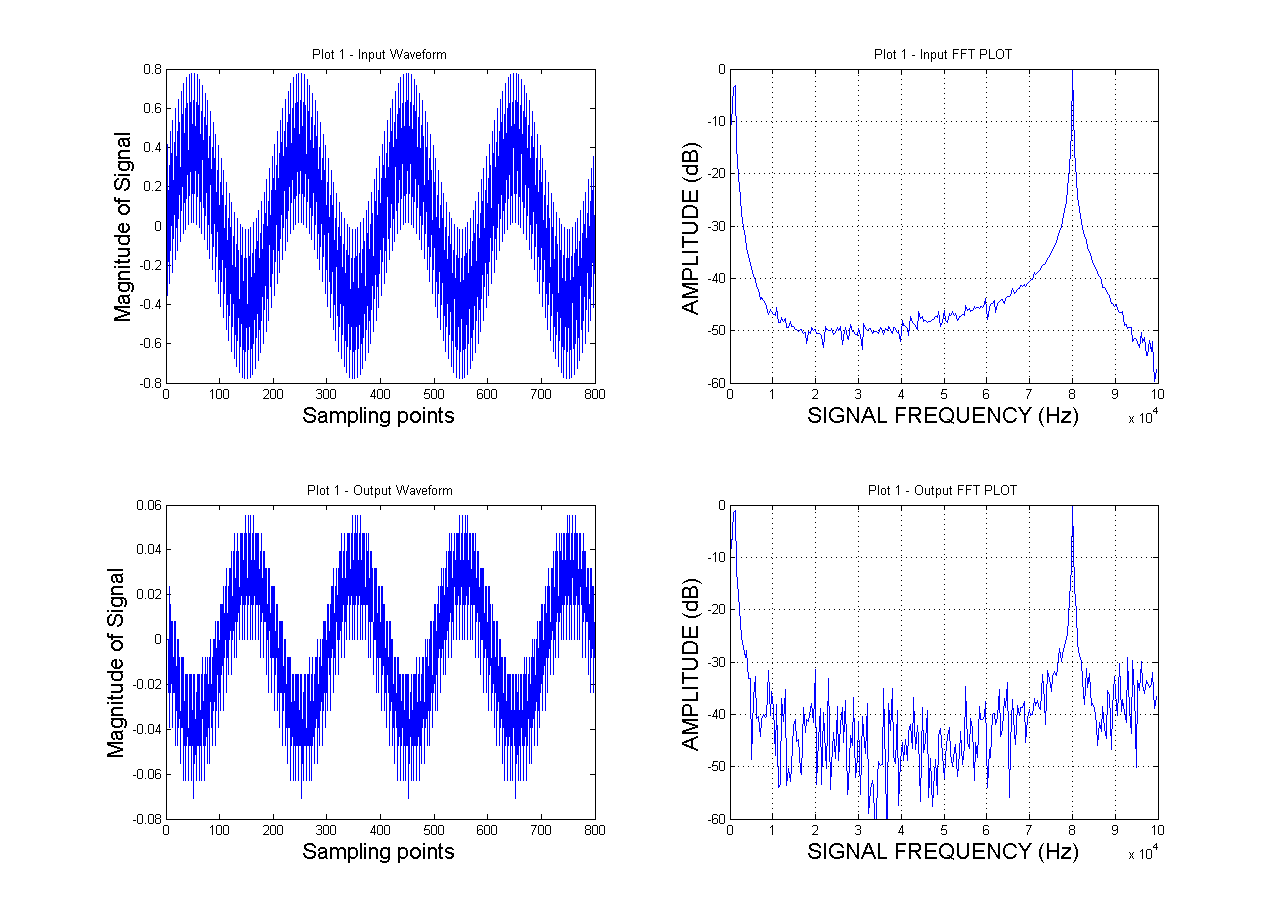
\includegraphics[scale=0.30]{plot1.png}} \\*
  \end{center}
  \caption{First Design Results}
  \label{fig:design1_results}
\end{figure}

